\documentclass[utf8, professionalfonts]{beamer}
\usetheme{Warsaw}

\usepackage[utf8]{inputenc}
\usepackage[english,russian]{babel}

\usepackage{url}
\usepackage{graphicx}
\usepackage{wrapfig}
\graphicspath{{./img/}{../img/}}

\title[Построение структурного выравнивания]{Инструменты построения и анализа структурного выравнивания молекул биополимеров для проекта UniPro UGENE}
\author[Кузнецов Алексей]{Кузнецов Алексей ФФ гр. 7312 \linebreak научный руководитель Фурсов М.Ю. UniPro}
\institute{Новосибирский Государственный Университет}
\date{\today}

\begin{document}

\begin{frame}
\titlepage
\end{frame}

\begin{frame}{Биологическая структура}
\begin{small}
Биологическая макромолекулярная структура -- это трехмерная модель молекулы.
\vspace{11pt}

Может быть получена следующими методами:
\begin{itemize}
        \item экспериментальными - NMR, X-Ray
        \item численного моделирования - <<предсказания структуры>>
\end{itemize}
\vspace{11pt}

Может включать также данные о связанной первичной структуре
   
\vspace{11pt}
Распространенный формат -- файлы PDB (\url{http://www.pdb.org})
\end{small}
\end{frame}

% Структурное выравнивание, что это такое
% Это попытка определить гомологичность двух белков
% на основе их третичной структуры
% Термин выравнивание взят по аналогии с выравниванием последовательностей
\begin{frame}{Структурное выравнивание}
\begin{columns}[c]
\column{0.45\linewidth}
    \center{\includegraphics[width=\linewidth]{wiki.png}}

\column{0.55\linewidth}
    Определение сходства (гомологии) биологических объектов по их \textbf{третичной} структуре.
    
    \vspace{11pt}
    Прямая аналогия с распространенной задачей поиска схожих последовательностей.

\end{columns}
\end{frame}

% Суть метода: выравниваем 2(попарное) или несколько(множественное) молекул
% минимизируя rmsd
\begin{frame}{Принцип}
\begin{figure}[h]
    \includegraphics[clip, trim=0 19.5cm 0 1cm, width=\linewidth]{method.pdf}
\end{figure}

Поиск трансформации ({\bf T}) для наилучшего выравнивания, минимизирующего {\bf RMSD} (root mean square deviation)
$ \operatorname{RMSD}(ref, mob) = \sqrt{ \dfrac{\sum_{i=1}^n \| \mathbf{\bar{x}}_{ref,i} -  \mathbf{\bar{x}}_{mob,i} \| ^2} {n} } $

\end{frame}

% Входные данные это третичная структура, попросту 3х-мерная модель
% может усугубляться всякими дополнительными данными
% Источники экспериментальные NMR, X-Ray; смоделированные
% обычно записывается в файлы формата PDB
% Результат rmsd и матрица пребразования
\begin{frame}{Результаты выравнивания}
Основные результаты работы алгоритма:
\begin{itemize}
	\item RMSD - root mean square deviation
	\item 4$\times$4 матрица преобразований модели - сдвиг, поворот
\end{itemize}	
\vspace{11pt}

Формат PDB позволяет записывать результаты выравнивания
\end{frame}


% Это важный инструмент структурной биологии
% Определение функционального назначения на основе структуры
% Сравнение белков с сильноразличающейся первичной структурой(аминокислотной последовательностью)
% Оценка алгоритмов предсказания структуры
\begin{frame}{Значение}
Структурное выравнивание имеет важное значение при решении ряда задач структурной биологии:
\begin{itemize}
    \item поиска гомологии среди биологических объектов
    \item классификации биополимеров по структурным особенностям
    \item определения функционального назначения биополимеров
    \item предсказания трехмерной структуры молекул биополимеров 
    \item и других...
\end{itemize}

\end{frame}


\begin{frame}{Недостатки существующих решений}
\begin{small}
\begin{itemize}
    \item Веб-сервисы (\textbf{DALI}, \textbf{VAST}): 
    \begin{itemize}
        \item[-] низкая производительность, значительное время ожидания
    \end{itemize}

    \item Узкоспециализированные утилиты (\textbf{FAST}, \textbf{MultiProt}):
    \begin{itemize}
        \item[-] необходимость наличия множества разнородных программ
        \item[-] проблема их совместной работы, <<протяжка результатов>>
    \end{itemize}

    \item Комплексные инструменты визуализации и анализа (\textbf{Swiss-PdbViewer}, \textbf{UCSF Chimera}, \textbf{PyMOL}):
    \begin{itemize}
        \item[-] недостаток средств визуализации, отсутствие специфичных стилей отображения и цветовых схем
        \item[-] слабая связь с инструментами анализа первичного и вторичного уровня структуры
    \end{itemize}

    \item Общие:
    \begin{itemize}
        \item[-] неудобный графический интерфейс или отсутствие такового
        \item[-] ограниченная поддержка платформ
    \end{itemize}

\end{itemize}
\end{small}
\end{frame}

% Пара слов о UGENE. Объединяет множество инструментов в одном формате.
% Уже имеет инструменты выравнивания последовательностей, визуализации макромолекул, ограниченную поддержку PDB
\begin{frame}{UGENE}
\begin{center}
\Large{UniPro UGENE -- это открытое ПО для работы молекулярного биолога}
\end{center}

% Слайд UGENE #1 - Цели проекта, скриншот
\begin{columns}
\column{0.5\linewidth}
	\center{\includegraphics[width=\linewidth]{screen.png}}
	
\column{0.5\linewidth}
	Цель проекта: Качественная интеграция существующих инструментов для биолога в единый графический и вычислительный интерфейс
	
\end{columns}
\end{frame}



% Цель: реализовать такой инструмент в продукте UniPro UGENE
% Задачи: построение, визуализация, импорт/экспорт, оформление, основа для дальнейшего развития
\begin{frame}{Цель работы}
\begin{center}
\Large Реализовать инструменты построения и визуализации структурного выравнивания на базе существующего алгоритма
\end{center}
\vspace{11pt}
Задачи
\begin{itemize}
    \item Обзор готовых решений и выбор подходящего алгоритма
    \item Интеграция алгоритма с инструментарием UGENE
    \item Реализация трехмерного визуализатора выравнивания
    \item Разработка графического пользовательского интерфейса
    \item Выделение общего API для алгоритмов выравнивания   
    \item Автоматизированное тестирование созданных компонентов
\end{itemize}
\end{frame}

\begin{frame}{Библиотека PTools}
    В качестве реализации выбран алгоритм выравнивания из библиотеки {\bf PTools} ({\it an opensource molecular docking library}), удовлетворяющей требованиям:
    \begin{itemize}
        \item Доступный исходный код и совместимая с GPL лицензия
        \item Язык реализации C/C++
        \item Переносимость, поддержка Linux, Win и Mac
        \item Четкая модульность
        \item Наличие документации
    \end{itemize}
\end{frame}


% Результаты
\begin{frame}{Результаты работы}
\begin{small}
\begin{itemize}
    \item Реализован инструмент построения структурного выравнивания на базе библиотеки PTools
    \item Решение успешно интегрировано с существующим инструментарием UGENE
    \item Реализована трехмерная визуализация выравнивания и GUI
    \item Написаны автоматические тесты, работа протестирована на платформах Linux, Win и Mac
    \item Как часть UGENE разработанные компоненты вошли поставку в дистрибутивов ОС Ubuntu Linux и Fedora Core
    \item Данная работа представлена на МНСК (Новосибирск, 2011)

\end{itemize}
\end{small}
\end{frame}


\begin{frame}{Визуализация}
\begin{figure}[h]
    \includegraphics[width=0.5\linewidth]{alignment-3TRX-vs-1XWC}
\end{figure}

\begin{center}
\begin{small}
Визуализация выравнивания молекул тиоредоксина человека~(\textbf{3TRX}) и~чернобрюхой~дрозофилы~(\textbf{1XWC})
\end{small}
\end{center}

\end{frame}


% Спасибо за внимание
\begin{frame}{Q\&A}
\begin{center} 
\LARGE{Спасибо за внимание!}
\end{center}
\end{frame}

\end{document}

% % Слайд с кучей алгоритмов, немногие из них существуют в виде законченных продуктов
% \begin{frame}{Существующие алгоритмы}
% \begin{center}
% \begin{small}
% MAMMOTH CE/CE-MC DaliLite VAST PrISM SSAP SARF2 KENOBI/K2 STAMP MASS SCALI DEJAVU SSM SHEBA LGA POSA PyMOL FATCAT Matras MAMMOTH-mult Protein3Dfit PRIDE FAST C-BOP ProFit TOPOFIT MUSTANG URMS LOCK LOCK 2 CBA TetraDA STRAP LOVOALIGN GANGSTA GANGSTA+ TM-align MatAlign Vorolign EXPRESSO CAALIGN YAKUSA BLOMAPS CLEPAPS TALI F MolCom MALECON FlexProt MultiProt CTSS CURVE Matt TopMatch SSGS Matchprot UCSF Chimera  FLASH RAPIDO ComSubstruct ProCKSI SARST Fr-TM-align TOPS+ COMPARISON TOPS++ FATCAT MolLoc FASE SABERTOOTH STON SALIGN MAX-PAIRS THESEUS TABLEAUSearch QP Tableau Search ProSMoS MISTRAL MSVNS for MaxCMO Structal ProBiS ALADYN SWAPSC SA Tableau Search
% \end{small}
% \end{center}
% \end{frame} 

% Слайд UGENE #2 - Преимущества, что уже есть
% \begin{frame}{Преимущества UGENE}
% 
% \begin{columns}[c]
%       \column{0.67\linewidth}
%               \begin{itemize}
%                       \item Проект активно развивается
%                       \item Объединяет десятки популярных инструментов биолога
%                       \item Более {\bf 10\textsuperscript{6}} строк кода, более {\bf 5000} автоматических тестов
%                       \item Платформы {\bf Windows}, {\bf Linux} и {\bf Mac}
%                       \item Входит в официальную поставку дистрибутивов {\bf Ubuntu} и {\bf Fedora}
%                       \item Сообщество {\bf $\sim$1000} пользователей
%                       \item Код доступен по лиценззи {\bf GPL} 
%                       \item публичный багтрекер, форум, видео-подкаст
%               \end{itemize}
%       
%       \column{0.4\linewidth}
%               \center{\includegraphics[width=0.8\linewidth]{gnu.png}}
%               \center{\includegraphics[width=0.8\linewidth]{platforms.png}}
% \end{columns}
% 
% \end{frame}